\documentclass[12pt,a4paper]{article}
\usepackage[utf8]{inputenc}
\usepackage{graphicx}
\usepackage{hyperref}
\usepackage{listings}
\usepackage{xcolor}
\usepackage{geometry}
\usepackage{longtable}
\usepackage{enumitem}
\usepackage{tikz}
\usetikzlibrary{shapes,arrows,positioning,fit,calc}

\geometry{margin=2.5cm}

\title{Museum Management Software\\Technical Documentation}
\author{Development Team}
\date{\today}

\begin{document}

\maketitle
\tableofcontents
\newpage

\section{Introduction}
This document provides comprehensive documentation for the Museum Management Software, including system architecture, maintenance procedures, and usage guidelines. This documentation covers every single file in the project and provides detailed information about their purpose, functionality, and usage.

\section{Project Overview}
The Museum Management Software is a Java-based desktop application built using Swing for the user interface. The system is designed to manage museum operations, including user authentication, administrative functions, and user-specific features.

\section{System Architecture}

\subsection{Frontend Architecture}
The frontend is built using Java Swing, providing a rich desktop application experience.

\begin{figure}[h]
\centering
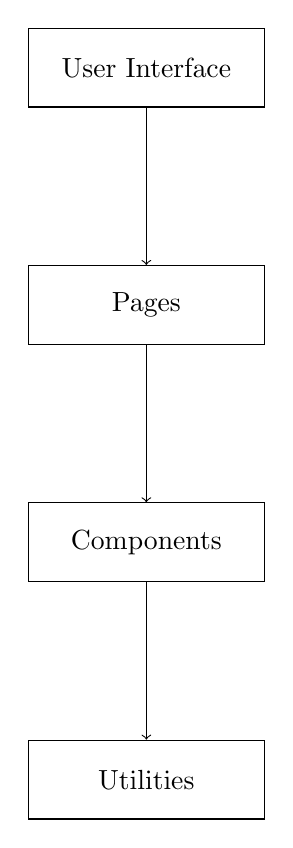
\begin{tikzpicture}[node distance=2cm]
    \node (ui) [rectangle, draw, minimum width=3cm, minimum height=1cm] {User Interface};
    \node (pages) [rectangle, draw, below=of ui, minimum width=3cm, minimum height=1cm] {Pages};
    \node (components) [rectangle, draw, below=of pages, minimum width=3cm, minimum height=1cm] {Components};
    \node (utils) [rectangle, draw, below=of components, minimum width=3cm, minimum height=1cm] {Utilities};
    
    \draw [->] (ui) -- (pages);
    \draw [->] (pages) -- (components);
    \draw [->] (components) -- (utils);
\end{tikzpicture}
\caption{Frontend Architecture Layers}
\end{figure}

\subsubsection{UI Framework}
\begin{itemize}
    \item \textbf{Technology Stack}
    \begin{itemize}
        \item Java Swing for UI components
        \item Custom UI components in \texttt{Components/} directory
        \item Event-driven architecture
        \item MVC pattern implementation
    \end{itemize}
    
    \item \textbf{Key Components}
    \begin{itemize}
        \item Custom cards for item display
        \item Navigation system
        \item Form components
        \item Data display widgets
    \end{itemize}
    
    \item \textbf{UI Organization}
    \begin{itemize}
        \item Role-based interfaces (Admin/User)
        \item Responsive layouts
        \item Consistent styling
        \item Accessibility features
    \end{itemize}
\end{itemize}

\subsubsection{User Interface Layers}
\begin{itemize}
    \item \textbf{Presentation Layer}
    \begin{itemize}
        \item \texttt{Pages/} directory containing all UI frames
        \item \texttt{Components/} directory for reusable UI elements
        \item Custom styling and theming
        \item Event handlers and listeners
    \end{itemize}
    
    \item \textbf{View Models}
    \begin{itemize}
        \item Data binding implementations
        \item State management
        \item UI update mechanisms
        \item Validation logic
    \end{itemize}
\end{itemize}

\subsection{Middleware Architecture}
The middleware layer handles business logic, data processing, and communication between frontend and backend.

\begin{figure}[h]
\centering
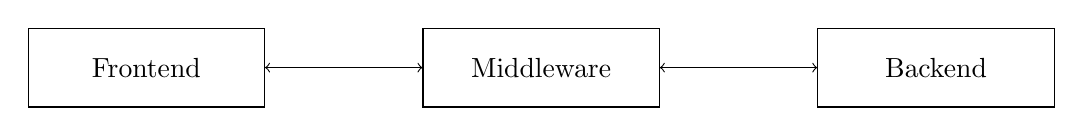
\begin{tikzpicture}[node distance=2cm]
    \node (frontend) [rectangle, draw, minimum width=3cm, minimum height=1cm] {Frontend};
    \node (middleware) [rectangle, draw, right=of frontend, minimum width=3cm, minimum height=1cm] {Middleware};
    \node (backend) [rectangle, draw, right=of middleware, minimum width=3cm, minimum height=1cm] {Backend};
    
    \draw [<->] (frontend) -- (middleware);
    \draw [<->] (middleware) -- (backend);
\end{tikzpicture}
\caption{Middleware Communication Flow}
\end{figure}

\subsubsection{Business Logic Layer}
\begin{itemize}
    \item \textbf{Core Components}
    \begin{itemize}
        \item \texttt{Components/Utilities/} for business logic
        \item Data validation and processing
        \item Business rules implementation
        \item State management
    \end{itemize}
    
    \item \textbf{Service Layer}
    \begin{itemize}
        \item Authentication services
        \item Data processing services
        \item Image handling services
        \item Search and filter services
    \end{itemize}
    
    \item \textbf{Data Access Layer}
    \begin{itemize}
        \item Database connection management
        \item Query execution
        \item Transaction handling
        \item Data mapping
    \end{itemize}
\end{itemize}

\subsubsection{Integration Layer}
\begin{itemize}
    \item \textbf{Data Transformation}
    \begin{itemize}
        \item Object-relational mapping
        \item Data format conversion
        \item Validation rules
        \item Error handling
    \end{itemize}
    
    \item \textbf{Communication}
    \begin{itemize}
        \item Frontend-backend communication
        \item Event propagation
        \item State synchronization
        \item Error propagation
    \end{itemize}
\end{itemize}

\subsection{Backend Architecture}
The backend is built on MySQL database with custom data processing utilities.

\begin{figure}[h]
\centering
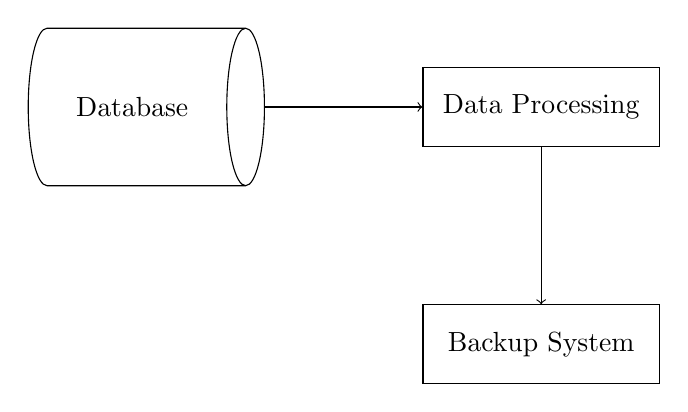
\begin{tikzpicture}[node distance=2cm]
    \node (db) [cylinder, draw, minimum width=2cm, minimum height=3cm] {Database};
    \node (processing) [rectangle, draw, right=of db, minimum width=3cm, minimum height=1cm] {Data Processing};
    \node (backup) [rectangle, draw, below=of processing, minimum width=3cm, minimum height=1cm] {Backup System};
    
    \draw [->] (db) -- (processing);
    \draw [->] (processing) -- (backup);
\end{tikzpicture}
\caption{Backend Architecture Components}
\end{figure}

\subsubsection{Database Layer}
\begin{itemize}
    \item \textbf{Database Design}
    \begin{itemize}
        \item MySQL database schema
        \item Table relationships
        \item Index optimization
        \item Constraint management
    \end{itemize}
    
    \item \textbf{Data Management}
    \begin{itemize}
        \item CRUD operations
        \item Transaction management
        \item Backup and recovery
        \item Data integrity
    \end{itemize}
    
    \item \textbf{Query Optimization}
    \begin{itemize}
        \item Indexed queries
        \item Stored procedures
        \item Query caching
        \item Performance monitoring
    \end{itemize}
\end{itemize}

\subsubsection{Data Processing}
\begin{itemize}
    \item \textbf{Data Tools}
    \begin{itemize}
        \item \texttt{get\_data.py} for data processing
        \item Data validation scripts
        \item Import/export utilities
        \item Data transformation tools
    \end{itemize}
    
    \item \textbf{Backup System}
    \begin{itemize}
        \item Automated backups
        \item Data recovery
        \item Version control
        \item Archive management
    \end{itemize}
\end{itemize}

\subsubsection{Security Layer}
\begin{itemize}
    \item \textbf{Authentication}
    \begin{itemize}
        \item User authentication
        \item Role-based access control
        \item Session management
        \item Password security
    \end{itemize}
    
    \item \textbf{Data Protection}
    \begin{itemize}
        \item Data encryption
        \item Secure communication
        \item Access logging
        \item Security monitoring
    \end{itemize}
\end{itemize}

\section{Connection System and Data Flow}

\subsection{Database Connection Architecture}
The application implements a centralized database connection system through the \texttt{DatabaseConnection} utility class.

\begin{figure}[h]
\centering
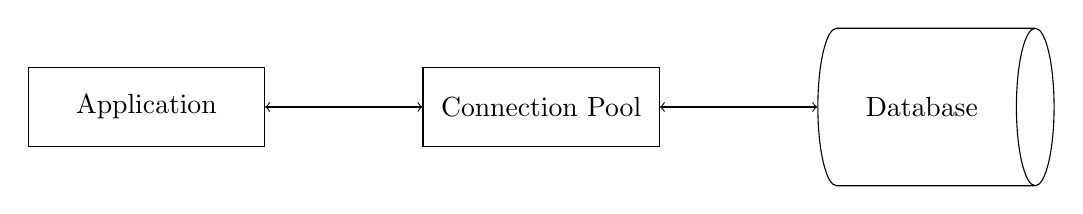
\begin{tikzpicture}[node distance=2cm]
    \node (app) [rectangle, draw, minimum width=3cm, minimum height=1cm] {Application};
    \node (pool) [rectangle, draw, right=of app, minimum width=3cm, minimum height=1cm] {Connection Pool};
    \node (db) [cylinder, draw, right=of pool, minimum width=2cm, minimum height=3cm] {Database};
    
    \draw [<->] (app) -- (pool);
    \draw [<->] (pool) -- (db);
\end{tikzpicture}
\caption{Database Connection Architecture}
\end{figure}

\subsection{Data Flow Examples}

\subsubsection{Collection Display Flow}
\begin{figure}[h]
\centering
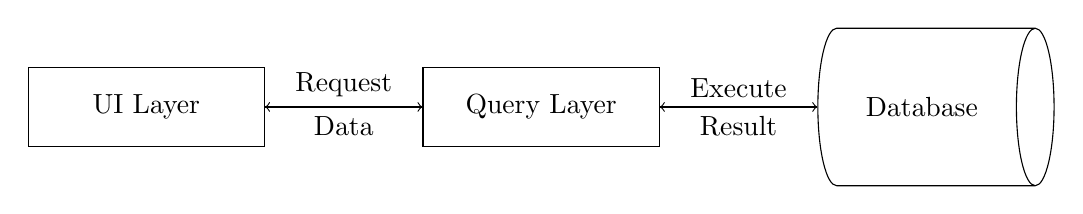
\begin{tikzpicture}[node distance=2cm]
    \node (ui) [rectangle, draw, minimum width=3cm, minimum height=1cm] {UI Layer};
    \node (query) [rectangle, draw, right=of ui, minimum width=3cm, minimum height=1cm] {Query Layer};
    \node (db) [cylinder, draw, right=of query, minimum width=2cm, minimum height=3cm] {Database};
    
    \draw [->] (ui) -- node[above] {Request} (query);
    \draw [->] (query) -- node[above] {Execute} (db);
    \draw [->] (db) -- node[below] {Result} (query);
    \draw [->] (query) -- node[below] {Data} (ui);
\end{tikzpicture}
\caption{Collection Display Data Flow}
\end{figure}

\begin{enumerate}
    \item \texttt{MuseumCollection.java} initiates data request
    \item Calls \texttt{ItemQueries.getCollectionItems()}
    \item \texttt{DatabaseConnection} executes query
    \item ResultSet returned to \texttt{MuseumCollection}
    \item Data processed by \texttt{ContainerPopulator}
    \item Displayed through \texttt{ItemCard} components
\end{enumerate}

\subsubsection{Item Management Flow}
\begin{enumerate}
    \item \texttt{AddItem.java} collects item data
    \item Validates through \texttt{validateItemInput()}
    \item Calls \texttt{ItemQueries.insertItem()}
    \item \texttt{DatabaseConnection} executes insert
    \item Transaction committed
    \item UI updated via \texttt{ContainerPopulator}
\end{enumerate}

\subsubsection{Search Implementation}
\begin{enumerate}
    \item \texttt{SearchBar.java} captures user input
    \item Triggers \texttt{ItemQueries.searchItems()}
    \item \texttt{DatabaseConnection} executes search query
    \item Results processed by \texttt{ContainerPopulator}
    \item Displayed in \texttt{MuseumCollection} view
\end{enumerate}

\subsection{Connection Management}

\begin{figure}[h]
\centering
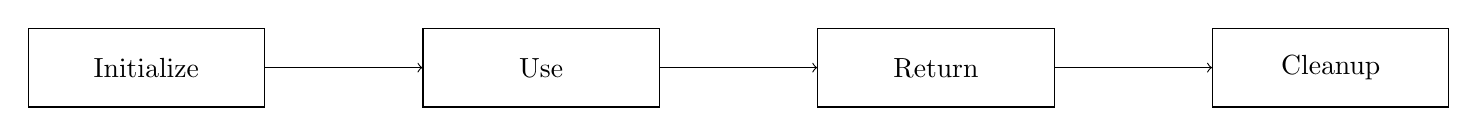
\begin{tikzpicture}[node distance=2cm]
    \node (init) [rectangle, draw, minimum width=3cm, minimum height=1cm] {Initialize};
    \node (use) [rectangle, draw, right=of init, minimum width=3cm, minimum height=1cm] {Use};
    \node (return) [rectangle, draw, right=of use, minimum width=3cm, minimum height=1cm] {Return};
    \node (clean) [rectangle, draw, right=of return, minimum width=3cm, minimum height=1cm] {Cleanup};
    
    \draw [->] (init) -- (use);
    \draw [->] (use) -- (return);
    \draw [->] (return) -- (clean);
\end{tikzpicture}
\caption{Connection Lifecycle}
\end{figure}

\subsubsection{Resource Handling}
\begin{itemize}
    \item \textbf{Connection Lifecycle}
    \begin{itemize}
        \item Connections obtained from pool
        \item Used for query execution
        \item Returned to pool after use
        \item Automatic cleanup on application exit
    \end{itemize}
    
    \item \textbf{Error Recovery}
    \begin{itemize}
        \item Connection timeout handling
        \item Automatic reconnection attempts
        \item Error logging and reporting
        \item User notification system
    \end{itemize}
\end{itemize}

\subsubsection{Performance Optimization}
\begin{itemize}
    \item \textbf{Connection Pooling}
    \begin{itemize}
        \item Fixed pool size management
        \item Connection reuse
        \item Idle connection cleanup
        \item Pool monitoring
    \end{itemize}
    
    \item \textbf{Query Optimization}
    \begin{itemize}
        \item Prepared statement caching
        \item Batch operation support
        \item ResultSet streaming
        \item Connection timeout settings
    \end{itemize}
\end{itemize}

\subsection{Data Access Patterns}

\subsubsection{Read Operations}
\begin{lstlisting}[language=Java]
// Example: Fetching collection items
public ResultSet getCollectionItems() {
    String query = ItemQueries.SELECT_ALL_ITEMS;
    return DatabaseConnection.executeQuery(query);
}

// Example: Searching items
public ResultSet searchItems(String searchTerm) {
    String query = ItemQueries.SEARCH_ITEMS;
    PreparedStatement stmt = DatabaseConnection.prepareStatement(query);
    stmt.setString(1, "%" + searchTerm + "%");
    return stmt.executeQuery();
}
\end{lstlisting}

\subsubsection{Write Operations}
\begin{lstlisting}[language=Java]
// Example: Adding new item
public boolean addItem(Item item) {
    String query = ItemQueries.INSERT_ITEM;
    PreparedStatement stmt = DatabaseConnection.prepareStatement(query);
    stmt.setString(1, item.getName());
    stmt.setString(2, item.getDescription());
    // ... set other parameters
    return stmt.executeUpdate() > 0;
}

// Example: Updating item
public boolean updateItem(Item item) {
    String query = ItemQueries.UPDATE_ITEM;
    PreparedStatement stmt = DatabaseConnection.prepareStatement(query);
    stmt.setString(1, item.getName());
    stmt.setString(2, item.getDescription());
    // ... set other parameters
    stmt.setInt(7, item.getId());
    return stmt.executeUpdate() > 0;
}
\end{lstlisting}

\subsection{Transaction Management}

\begin{figure}[h]
\centering
\begin{tikzpicture}[node distance=2cm]
    \node (start) [rectangle, draw, minimum width=3cm, minimum height=1cm] {Start Transaction};
    \node (exec) [rectangle, draw, right=of start, minimum width=3cm, minimum height=1cm] {Execute Operations};
    \node (check) [diamond, draw, right=of exec, minimum width=3cm, minimum height=2cm] {Success?};
    \node (commit) [rectangle, draw, above=of check, minimum width=3cm, minimum height=1cm] {Commit};
    \node (rollback) [rectangle, draw, below=of check, minimum width=3cm, minimum height=1cm] {Rollback};
    
    \draw [->] (start) -- (exec);
    \draw [->] (exec) -- (check);
    \draw [->] (check) -- node[left] {Yes} (commit);
    \draw [->] (check) -- node[left] {No} (rollback);
\end{tikzpicture}
\caption{Transaction Flow}
\end{figure}

\subsubsection{Transaction Patterns}
\begin{itemize}
    \item \textbf{Simple Transactions}
    \begin{itemize}
        \item Single operation commits
        \item Automatic rollback on failure
        \item Connection state management
    \end{itemize}
    
    \item \textbf{Complex Transactions}
    \begin{itemize}
        \item Multiple operation batches
        \item Manual commit control
        \item Savepoint management
        \item Rollback handling
    \end{itemize}
\end{itemize}

\subsubsection{Error Handling}
\begin{itemize}
    \item \textbf{Database Errors}
    \begin{itemize}
        \item SQL exception handling
        \item Connection failure recovery
        \item Transaction rollback
        \item User notification
    \end{itemize}
    
    \item \textbf{Application Errors}
    \begin{itemize}
        \item Data validation errors
        \item Business rule violations
        \item Resource cleanup
        \item Error logging
    \end{itemize}
\end{itemize}

\section{Project Structure}

\begin{figure}[h]
\centering
\begin{tikzpicture}[node distance=2cm]
    \node (root) [rectangle, draw, minimum width=3cm, minimum height=1cm] {Project Root};
    \node (src) [rectangle, draw, below=of root, minimum width=3cm, minimum height=1cm] {src/};
    \node (build) [rectangle, draw, right=of src, minimum width=3cm, minimum height=1cm] {build/};
    \node (lib) [rectangle, draw, left=of src, minimum width=3cm, minimum height=1cm] {lib/};
    
    \draw [->] (root) -- (src);
    \draw [->] (root) -- (build);
    \draw [->] (root) -- (lib);
\end{tikzpicture}
\caption{Project Directory Structure}
\end{figure}

The project follows a well-organized directory structure:

\subsection{Root Directory Contents}
\begin{itemize}
    \item \texttt{src/} - Source code directory
    \item \texttt{build/} - Build output directory
    \item \texttt{lib/} - External libraries
    \item \texttt{dataBackup/} - Database backup directory
    \item \texttt{.idea/} - IntelliJ IDEA configuration
    \item \texttt{out/} - Compiled output directory
    \item \texttt{build.xml} - Ant build configuration
    \item \texttt{README.md} - Project overview
    \item \texttt{.gitignore} - Git ignore rules
\end{itemize}

\section{Source Code Organization}

\subsection{Main Application}
\subsubsection{Main.java}
Location: \texttt{src/com/app/Main.java}
Size: 1.6KB
Lines: 56

\paragraph{Purpose}
The main entry point of the application that initializes the system and manages window navigation.

\paragraph{Key Components}
\begin{itemize}
    \item Window stack management
    \item Application initialization
    \item Navigation control
\end{itemize}

\paragraph{Methods}
\begin{itemize}
    \item \texttt{main(String[] args)} - Application entry point
    \item \texttt{showWindow(JFrame newWindow)} - Displays new window
    \item \texttt{goBack()} - Handles back navigation
    \item \texttt{clearStack()} - Clears window stack
\end{itemize}

\subsection{Components Directory}
Located in \texttt{src/Components/}, contains reusable UI components and utilities.

\subsubsection{Utilities}
\paragraph{DatabaseConnection.java}
Location: \texttt{src/Components/Utilities/DatabaseConnection.java}
Size: 1.7KB
Lines: 52

\paragraph{Purpose}
Manages database connections and provides database access methods.

\paragraph{Key Features}
\begin{itemize}
    \item Connection pooling
    \item Query execution
    \item Connection management
    \item Error handling
\end{itemize}

\paragraph{Methods}
\begin{itemize}
    \item \texttt{getConnection()} - Establishes database connection
    \item \texttt{executeQuery(String query)} - Executes SQL queries
    \item \texttt{closeConnection()} - Closes database connection
\end{itemize}

\paragraph{Config.java}
Location: \texttt{src/Components/Utilities/Config.java}
Size: 1.5KB
Lines: 55

\paragraph{Purpose}
Manages application configuration and settings.

\paragraph{Key Features}
\begin{itemize}
    \item Configuration loading
    \item Settings management
    \item Environment variables
\end{itemize}

\paragraph{ImageResizer.java}
Location: \texttt{src/Components/Utilities/ImageResizer.java}
Size: 4.8KB
Lines: 107

\paragraph{Purpose}
Handles image processing and resizing for museum items.

\paragraph{Key Features}
\begin{itemize}
    \item Image resizing
    \item Format conversion
    \item Quality optimization
    \item Thumbnail generation
\end{itemize}

\paragraph{Methods}
\begin{itemize}
    \item \texttt{resizeImage(Image original, int width, int height)}
    \item \texttt{createThumbnail(Image original)}
    \item \texttt{optimizeImage(Image image)}
\end{itemize}

\paragraph{ItemQueries.java}
Location: \texttt{src/Components/Utilities/ItemQueries.java}
Size: 3.3KB
Lines: 82

\paragraph{Purpose}
Contains SQL queries for item management.

\paragraph{Key Features}
\begin{itemize}
    \item CRUD operations
    \item Search queries
    \item Filter queries
    \item Join operations
\end{itemize}

\paragraph{ContainerPopulator.java}
Location: \texttt{src/Components/Utilities/ContainerPopulator.java}
Size: 5.8KB
Lines: 130

\paragraph{Purpose}
Manages dynamic content population in UI containers.

\paragraph{Key Features}
\begin{itemize}
    \item Dynamic content loading
    \item Container management
    \item Layout handling
    \item Event binding
\end{itemize}

\paragraph{StatsCounter.java}
Location: \texttt{src/Components/Utilities/StatsCounter.java}
Size: 2.2KB
Lines: 67

\paragraph{Purpose}
Tracks and displays system statistics.

\paragraph{Key Features}
\begin{itemize}
    \item Counter management
    \item Statistics calculation
    \item Data aggregation
    \item Display formatting
\end{itemize}

\paragraph{CustomScrollBar.java}
Location: \texttt{src/Components/Utilities/CustomScrollBar.java}
Size: 1.5KB
Lines: 43

\paragraph{Purpose}
Custom scrollbar implementation for consistent UI.

\paragraph{Key Features}
\begin{itemize}
    \item Custom styling
    \item Smooth scrolling
    \item Event handling
    \item Size management
\end{itemize}

\subsubsection{Cards}
\paragraph{NavigationBar.java}
Location: \texttt{src/Components/Cards/NavigationBar.java}
Size: 14KB
Lines: 277

\paragraph{Purpose}
Main navigation component for the application.

\paragraph{Key Features}
\begin{itemize}
    \item Menu management
    \item Navigation handling
    \item User role adaptation
    \item Dynamic updates
\end{itemize}

\paragraph{SearchBar.java}
Location: \texttt{src/Components/Cards/SearchBar.java}
Size: 2.9KB
Lines: 76

\paragraph{Purpose}
Search functionality implementation.

\paragraph{Key Features}
\begin{itemize}
    \item Real-time search
    \item Filter options
    \item Search history
    \item Results display
\end{itemize}

\subsubsection{Collection Cards}
\paragraph{ItemCard.java}
Location: \texttt{src/Components/Cards/Collection/ItemCard.java}
Size: 7.9KB
Lines: 190

\paragraph{Purpose}
Displays individual museum items in the collection.

\paragraph{Key Features}
\begin{itemize}
    \item Item display
    \item Image handling
    \item Information layout
    \item Interaction handling
\end{itemize}

\paragraph{RecentlyAddedCard.java}
Location: \texttt{src/Components/Cards/Collection/RecentlyAddedCard.java}
Size: 9.1KB
Lines: 201

\paragraph{Purpose}
Displays recently added museum items.

\paragraph{Key Features}
\begin{itemize}
    \item Recent items display
    \item Time-based sorting
    \item Quick access
    \item Update handling
\end{itemize}

\paragraph{RecentlyAddedContainer.java}
Location: \texttt{src/Components/Cards/Collection/RecentlyAddedContainer.java}
Size: 6.8KB
Lines: 181

\paragraph{Purpose}
Container for recently added items.

\paragraph{Key Features}
\begin{itemize}
    \item Layout management
    \item Card organization
    \item Scroll handling
    \item Update management
\end{itemize}

\paragraph{MuseumCollection.java}
Location: \texttt{src/Components/Cards/Collection/MuseumCollection.java}
Size: 12KB
Lines: 323

\paragraph{Purpose}
Main collection display component.

\paragraph{Key Features}
\begin{itemize}
    \item Collection display
    \item Filtering
    \item Sorting
    \item Pagination
\end{itemize}

\section{Pages Directory}
Located in \texttt{src/Pages/}, contains all application pages organized by user role.

\subsection{Login Pages}
\subsubsection{LoginFrame.java}
Location: \texttt{src/Pages/Login/LoginFrame.java}
Size: 9.4KB
Lines: 236

\paragraph{Purpose}
Main login interface for user authentication.

\paragraph{Key Features}
\begin{itemize}
    \item User authentication
    \item Password validation
    \item Session management
    \item Error handling
\end{itemize}

\paragraph{Methods}
\begin{itemize}
    \item \texttt{authenticateUser()}
    \item \texttt{validateInput()}
    \item \texttt{initializeSession()}
    \item \texttt{handleLoginError()}
\end{itemize}

\subsubsection{RegisterFrame.java}
Location: \texttt{src/Pages/Login/RegisterFrame.java}
Size: 10KB
Lines: 252

\paragraph{Purpose}
New user registration interface.

\paragraph{Key Features}
\begin{itemize}
    \item User registration
    \item Input validation
    \item Account creation
    \item Error handling
\end{itemize}

\paragraph{Methods}
\begin{itemize}
    \item \texttt{validateRegistration()}
    \item \texttt{createUserAccount()}
    \item \texttt{handleRegistrationError()}
    \item \texttt{checkUsernameAvailability()}
\end{itemize}

\subsection{Admin Pages}
\subsubsection{Dashboard.java}
Location: \texttt{src/Pages/Admin/Dashboard.java}
Size: 24KB
Lines: 444

\paragraph{Purpose}
Main admin control panel.

\paragraph{Key Features}
\begin{itemize}
    \item System statistics
    \item Quick access functions
    \item Activity monitoring
    \item Alert management
\end{itemize}

\paragraph{Methods}
\begin{itemize}
    \item \texttt{loadStatistics()}
    \item \texttt{updateDashboard()}
    \item \texttt{handleAlerts()}
    \item \texttt{manageQuickAccess()}
\end{itemize}

\subsubsection{Inventory.java}
Location: \texttt{src/Pages/Admin/Inventory.java}
Size: 9.0KB
Lines: 235

\paragraph{Purpose}
Inventory management interface.

\paragraph{Key Features}
\begin{itemize}
    \item Item listing
    \item Search functionality
    \item Filter management
    \item Item operations
\end{itemize}

\paragraph{Methods}
\begin{itemize}
    \item \texttt{loadInventory()}
    \item \texttt{searchItems()}
    \item \texttt{filterItems()}
    \item \texttt{updateInventory()}
\end{itemize}

\subsubsection{AddItem.java}
Location: \texttt{src/Pages/Admin/AddItem.java}
Size: 8.2KB
Lines: 222

\paragraph{Purpose}
Interface for adding new items to the collection.

\paragraph{Key Features}
\begin{itemize}
    \item Item input forms
    \item Image upload
    \item Category selection
    \item Location assignment
\end{itemize}

\paragraph{Methods}
\begin{itemize}
    \item \texttt{validateItemInput()}
    \item \texttt{handleImageUpload()}
    \item \texttt{saveNewItem()}
    \item \texttt{assignLocation()}
\end{itemize}

\subsubsection{EditItem.java}
Location: \texttt{src/Pages/Admin/EditItem.java}
Size: 8.1KB
Lines: 225

\paragraph{Purpose}
Interface for modifying existing items.

\paragraph{Key Features}
\begin{itemize}
    \item Item editing
    \item Image management
    \item Status updates
    \item Metadata editing
\end{itemize}

\paragraph{Methods}
\begin{itemize}
    \item \texttt{loadItemData()}
    \item \texttt{updateItem()}
    \item \texttt{handleImageUpdate()}
    \item \texttt{validateChanges()}
\end{itemize}

\subsubsection{Suggestions.java}
Location: \texttt{src/Pages/Admin/Suggestions.java}
Size: 12KB
Lines: 283

\paragraph{Purpose}
User suggestion management interface.

\paragraph{Key Features}
\begin{itemize}
    \item Suggestion review
    \item Status management
    \item Response handling
    \item Filtering options
\end{itemize}

\paragraph{Methods}
\begin{itemize}
    \item \texttt{loadSuggestions()}
    \item \texttt{updateStatus()}
    \item \texttt{sendResponse()}
    \item \texttt{filterSuggestions()}
\end{itemize}

\subsection{User Pages}
\subsubsection{HomePage.java}
Location: \texttt{src/Pages/User/HomePage.java}
Size: 33KB
Lines: 784

\paragraph{Purpose}
Main user interface.

\paragraph{Key Features}
\begin{itemize}
    \item Featured items
    \item Navigation
    \item Personalized content
    \item Quick access
\end{itemize}

\paragraph{Methods}
\begin{itemize}
    \item \texttt{loadFeaturedItems()}
    \item \texttt{updatePersonalizedContent()}
    \item \texttt{handleNavigation()}
    \item \texttt{initializeQuickAccess()}
\end{itemize}

\subsubsection{MuseumCollection.java}
Location: \texttt{src/Pages/User/MuseumCollection.java}
Size: 22KB
Lines: 489

\paragraph{Purpose}
Collection browsing interface.

\paragraph{Key Features}
\begin{itemize}
    \item Collection display
    \item Search functionality
    \item Category filtering
    \item Pagination
\end{itemize}

\paragraph{Methods}
\begin{itemize}
    \item \texttt{loadCollection()}
    \item \texttt{handleSearch()}
    \item \texttt{applyFilters()}
    \item \texttt{managePagination()}
\end{itemize}

\subsubsection{ItemDisplay.java}
Location: \texttt{src/Pages/User/ItemDisplay.java}
Size: 14KB
Lines: 350

\paragraph{Purpose}
Detailed item view interface.

\paragraph{Key Features}
\begin{itemize}
    \item Item details
    \item Image gallery
    \item Related items
    \item Information display
\end{itemize}

\paragraph{Methods}
\begin{itemize}
    \item \texttt{loadItemDetails()}
    \item \texttt{displayImages()}
    \item \texttt{findRelatedItems()}
    \item \texttt{formatInformation()}
\end{itemize}

\subsubsection{ItemProfile.java}
Location: \texttt{src/Pages/User/ItemProfile.java}
Size: 13KB
Lines: 297

\paragraph{Purpose}
Comprehensive item information display.

\paragraph{Key Features}
\begin{itemize}
    \item Historical information
    \item Conservation status
    \item Exhibition history
    \item Detailed metadata
\end{itemize}

\paragraph{Methods}
\begin{itemize}
    \item \texttt{loadHistory()}
    \item \texttt{updateConservationStatus()}
    \item \texttt{displayExhibitionHistory()}
    \item \texttt{formatMetadata()}
\end{itemize}

\subsubsection{SuggestionForm.java}
Location: \texttt{src/Pages/User/SuggestionForm.java}
Size: 9.1KB
Lines: 256

\paragraph{Purpose}
User feedback submission interface.

\paragraph{Key Features}
\begin{itemize}
    \item Form input
    \item Category selection
    \item Priority assignment
    \item Submission handling
\end{itemize}

\paragraph{Methods}
\begin{itemize}
    \item \texttt{validateForm()}
    \item \texttt{handleSubmission()}
    \item \texttt{assignPriority()}
    \item \texttt{selectCategory()}
\end{itemize}

\subsubsection{SuggestionTable.java}
Location: \texttt{src/Pages/User/SuggestionTable.java}
Size: 6.5KB
Lines: 184

\paragraph{Purpose}
User suggestion history display.

\paragraph{Key Features}
\begin{itemize}
    \item Suggestion listing
    \item Status display
    \item Response viewing
    \item Filtering options
\end{itemize}

\paragraph{Methods}
\begin{itemize}
    \item \texttt{loadSuggestions()}
    \item \texttt{displayStatus()}
    \item \texttt{showResponses()}
    \item \texttt{applyFilters()}
\end{itemize}

\section{Build System}
\subsection{build.xml}
Location: \texttt{build.xml}
Size: 1.9KB
Lines: 54

\paragraph{Purpose}
Ant build configuration file.

\paragraph{Key Features}
\begin{itemize}
    \item Build targets
    \item Dependency management
    \item Compilation settings
    \item Deployment configuration
\end{itemize}

\paragraph{Build Targets}
\begin{itemize}
    \item \texttt{clean} - Removes build artifacts
    \item \texttt{compile} - Compiles source files
    \item \texttt{jar} - Creates executable JAR
    \item \texttt{run} - Compiles and runs application
\end{itemize}

\section{Database}
\subsection{museum\_insert\_queries.sql}
Location: \texttt{src/tools/museum\_insert\_queries.sql}
Size: 541KB
Lines: 8477

\paragraph{Purpose}
Database initialization and data insertion scripts.

\paragraph{Key Features}
\begin{itemize}
    \item Table creation
    \item Data insertion
    \item Index creation
    \item Constraint definition
\end{itemize}

\subsection{get\_data.py}
Location: \texttt{src/tools/get\_data.py}
Size: 8.5KB
Lines: 180

\paragraph{Purpose}
Data processing and extraction utility.

\paragraph{Key Features}
\begin{itemize}
    \item Data extraction
    \item Format conversion
    \item Data validation
    \item Export functionality
\end{itemize}

\section{Maintenance and Updates}

\subsection{Code Maintenance}
\begin{enumerate}
    \item Follow the existing package structure
    \item Maintain separation of concerns
    \item Use the window stack for navigation
    \item Keep UI components in the Components directory
    \item Follow Java coding conventions
    \item Document all new features
    \item Test thoroughly before deployment
\end{enumerate}

\subsection{Database Maintenance}
\begin{enumerate}
    \item Regular backups using the backup functionality
    \item Monitor database performance
    \item Update database schema using provided SQL scripts
    \item Maintain data integrity
    \item Optimize queries
    \item Monitor storage usage
\end{enumerate}

\section{Usage Guidelines}

\subsection{Installation}
\begin{enumerate}
    \item Ensure Java Runtime Environment is installed
    \item Install MySQL Server
    \item Run database initialization scripts
    \item Build the project using Ant
    \item Configure database connection
    \item Set up backup directory
\end{enumerate}

\subsection{Running the Application}
\begin{enumerate}
    \item Execute the JAR file or use Ant run target
    \item Login with appropriate credentials
    \item Navigate through the application using the provided interface
    \item Follow role-specific guidelines
    \item Use provided help resources
\end{enumerate}

\section{Troubleshooting}
Common issues and solutions:
\begin{itemize}
    \item Database connection issues - Check MySQL service and credentials
    \item UI rendering problems - Verify Java version compatibility
    \item Build failures - Ensure all dependencies are present
    \item Performance issues - Check system resources
    \item Data inconsistencies - Verify database integrity
\end{itemize}

\section{Development Guidelines}
\begin{itemize}
    \item Follow Java coding conventions
    \item Document new features and changes
    \item Test thoroughly before deployment
    \item Maintain backup of critical data
    \item Use version control effectively
    \item Follow security best practices
\end{itemize}

\section{Conclusion}
This documentation provides a comprehensive guide to the Museum Management Software. For additional support or clarification, please contact the development team.

\section{Architectural Layer Classification}

\subsection{Frontend Layer}
The frontend layer consists of all UI-related components and pages:

\subsubsection{Pages}
\begin{itemize}
    \item \texttt{src/Pages/Login/}
    \begin{itemize}
        \item \texttt{LoginFrame.java} - Login interface
        \item \texttt{RegisterFrame.java} - Registration interface
    \end{itemize}
    
    \item \texttt{src/Pages/Admin/}
    \begin{itemize}
        \item \texttt{Dashboard.java} - Admin control panel
        \item \texttt{Inventory.java} - Inventory management
        \item \texttt{AddItem.java} - Item addition interface
        \item \texttt{EditItem.java} - Item editing interface
        \item \texttt{Suggestions.java} - Suggestion management
    \end{itemize}
    
    \item \texttt{src/Pages/User/}
    \begin{itemize}
        \item \texttt{HomePage.java} - User home interface
        \item \texttt{MuseumCollection.java} - Collection browsing
        \item \texttt{ItemDisplay.java} - Item details view
        \item \texttt{ItemProfile.java} - Item profile view
        \item \texttt{SuggestionForm.java} - Suggestion submission
        \item \texttt{SuggestionTable.java} - Suggestion history
    \end{itemize}
\end{itemize}

\subsubsection{UI Components}
\begin{itemize}
    \item \texttt{src/Components/Cards/}
    \begin{itemize}
        \item \texttt{NavigationBar.java} - Main navigation
        \item \texttt{SearchBar.java} - Search functionality
        \item \texttt{Collection/ItemCard.java} - Item display card
        \item \texttt{Collection/RecentlyAddedCard.java} - Recent items card
        \item \texttt{Collection/RecentlyAddedContainer.java} - Recent items container
        \item \texttt{Collection/MuseumCollection.java} - Collection display
    \end{itemize}
    
    \item \texttt{src/Components/Utilities/}
    \begin{itemize}
        \item \texttt{CustomScrollBar.java} - Custom UI scrollbar
        \item \texttt{ContainerPopulator.java} - Dynamic content population
    \end{itemize}
\end{itemize}

\subsection{Middleware Layer}
The middleware layer handles business logic and data processing:

\begin{itemize}
    \item \texttt{src/Components/Utilities/}
    \begin{itemize}
        \item \texttt{ImageResizer.java} - Image processing
        \item \texttt{StatsCounter.java} - Statistics management
        \item \texttt{Config.java} - Configuration management
    \end{itemize}
    
    \item \texttt{src/com/app/}
    \begin{itemize}
        \item \texttt{Main.java} - Application entry point and navigation
    \end{itemize}
\end{itemize}

\subsection{Backend Layer}
The backend layer manages data storage and database operations:

\begin{itemize}
    \item \texttt{src/Components/Utilities/}
    \begin{itemize}
        \item \texttt{DatabaseConnection.java} - Database connection management
        \item \texttt{ItemQueries.java} - Database queries
    \end{itemize}
    
    \item \texttt{src/tools/}
    \begin{itemize}
        \item \texttt{museum\_insert\_queries.sql} - Database schema and data
        \item \texttt{get\_data.py} - Data processing utility
    \end{itemize}
    
    \item \texttt{dataBackup/} - Database backup directory
\end{itemize}

\subsection{Configuration Files}
\begin{itemize}
    \item \texttt{build.xml} - Build configuration
    \item \texttt{README.md} - Project documentation
    \item \texttt{.gitignore} - Version control configuration
    \item \texttt{Museum Management Software - Project Files.iml} - Project configuration
\end{itemize}

\end{document} 